%%%%%%%%%%%%%%%%%%%%%%%%%%%%%%%%%%%%%%%%%
% FRI Data Science_report LaTeX Template
% Version 1.0 (28/1/2020)
% 
% Jure Demšar (jure.demsar@fri.uni-lj.si)
%
% Based on MicromouseSymp article template by:
% Mathias Legrand (legrand.mathias@gmail.com) 
% With extensive modifications by:
% Antonio Valente (antonio.luis.valente@gmail.com)
%
% License:
% CC BY-NC-SA 3.0 (http://creativecommons.org/licenses/by-nc-sa/3.0/)
%
%%%%%%%%%%%%%%%%%%%%%%%%%%%%%%%%%%%%%%%%%


%----------------------------------------------------------------------------------------
%	PACKAGES AND OTHER DOCUMENT CONFIGURATIONS
%----------------------------------------------------------------------------------------
\documentclass[fleqn,moreauthors,10pt]{ds_report}
\usepackage[english]{babel}

\graphicspath{{fig/}}




%----------------------------------------------------------------------------------------
%	ARTICLE INFORMATION
%----------------------------------------------------------------------------------------

% Header
\JournalInfo{FRI Natural language processing course 2021}

% Interim or final report
\Archive{Project report} 
%\Archive{Final report} 

% Article title
\PaperTitle{Offensive language exploratory analysis} 

% Authors (student competitors) and their info
\Authors{Matic Fučka, Anže Alič and Aljaž M. Eržen}

% Advisors
\affiliation{\textit{Advisors: Slavko Žitnik}}

% Keywords
\Keywords{Natural language processing, Statistical methods and hate speech}
\newcommand{\keywordname}{Keywords}


%----------------------------------------------------------------------------------------
%	ABSTRACT
%----------------------------------------------------------------------------------------

\Abstract{
In this report we present some insights into the basic construction of different sections of hate speech. We used different statistical methods to find most important words. We also used some traditional natural language processing methods and some non contextual neural approaches to finde the relationships between the classes of hate speech. % Pomoje je treba dodati sem se kak rezultat
}

%----------------------------------------------------------------------------------------

\begin{document}

% Makes all text pages the same height
\flushbottom 

% Print the title and abstract box
\maketitle 

% Removes page numbering from the first page
\thispagestyle{empty} 

%----------------------------------------------------------------------------------------
%	ARTICLE CONTENTS
%----------------------------------------------------------------------------------------

\section*{Introduction}
The main objective of this assignment is to give a better understanding of the basic construction and the relationship of different subareas of offensive language.

First we constructed a dataset of hate speech with different labels with the use of different hate speech datasets which included text which were qualified under different subareas of hate speech by different reaserchers in the field. Then we preprocessed the corpus so we received the stems of each word.

After the construction of the dataset we tackled the problem of analysis by extracting the most important words for each label given to us by using some traditional natural language processing (NLP), such as TF-IDF and n-grams, methods and some statistical methods, such as Pearson $\chi^2$ test.

With the extracted words we head onto the calculation of different embeddings for these words or texts. Once we got the embeddings we tried different clustering methods such as PCA, TSNE, etc. to group these embeddings. We also discussed the results of the approaches that yielded some useful information.


%------------------------------------------------

\section*{Methods}

\subsection*{Corpus merging}

We extended our dataset selection to 7 different datasets, together including 19 different labels for hate speech types and a ``not hate speech'' label. Collections sources include Twitter \cite{20_twitter, 32_twitter, vulgar-twitter, 25_twitter}, Facebook \cite{16_facebook}, Wikipedia comments \cite{kaggle-jigsaw} and Reddit \cite{zenodo}. Which dataset contained which labels and how many of them can be seen in Table~\ref{tab:sentiment-source}.
% abusive appearance_harassment disrespectful fearful hateful homophobic insult intelligence_harassment misogynistic obscene offensive political_harassment profanity racist severe_toxic sexual_harassment threat toxic vulgar none
It should be noted that some labels were present only in one dataset and some datasets had all documents labeled with a single label. Documents of one dataset were labeled with multiple labels, which we solved by mapping each of the documents into multiple replicas where each of them was labeled with one of initial labels (e.g. document labeled as \texttt{fearful\_abusive\_hateful} was replicated into 3 documents with labels \texttt{fearful}, \texttt{abusive}, and \texttt{hateful}).

Some datasets did not label \textit{type of hate speech} but labeled sentiment, directness, target, group or some other property. From this we interpolated our \textit{type of hate speech} using best effort approximations. For example, we labeled \texttt{hostile} sentiment with target \texttt{women} as \texttt{misogynistic} and target \texttt{sexual\_orientation} with \texttt{homophobic}. This relabeling is not ideal due to gap between the meanings, which is why we interpolated only labels that were not found anywhere else, so there would not be clash between meanings of a single label.

Our process of merging datasets is not ideal because replicating multi-label documents introduces high correlation between labels from this dataset. Also, if labels are provided by only one dataset, we are essentially only comparing the biases of the datasets. This bias is composed of annotator's bias in interpretation of some \textit{type of hate speech} (which is what we are after) and other biases such as collection source of the dataset or preprocessing techniques. This is why results of our analysis cannot necessarily confirm correlation between labels as correlations between \textit{types of hate speech}, because it may be caused by other biases.

\subsection*{Data preprocessing}
Text in our corpus is mostly from from sources such as twitter. So we have to remove emojis, tags etc. We first replace emojis with corresponding words (e.g. replace fire emoji with word ¨fire"). Than we used special twitter tokenizer to tokenize text into tokens. We remove token which correspond to urls, mentions, unknown emojis or hashtags. On the end we stem each token with Snowball stemmer.


%\subsection*{Pearson $\chi^2$ test}

%The Pearson $\chi^2$ test is an statistical hypothesis, which determines whether there is a statistically significance between the expected and the observed frequencies. If we define $E_G(w)$ the expected frequency of the word $w$ in some general corpus $G$ and $O_R(w)$ the observed frequency in specific corpus $R$ then the value of the Pearson $\chi^2$ test for word w (which we dub $P_R(w)$) is as follows:
% \begin{equation}
%     P_R(w) = \frac{(E_G(w)-O_R(w))^2}{E_G(w)}
% \end{equation}
% If the value of the Pearson $\chi^2$ test $P_R(w)$ exceeds 3.84 for some word $w$ in a specific corpus $R$ then we are able to say with a 95\% certainty that the word $w$ is statistically significant for the corpus $R$.

% \subsection*{FastText}
% FastText is a non-contextual neural model for learning word embeddings in an either supervised or an unsupervised manner. It is an extension of the word2vec model but instead of learning the vectors for words directly it learns each word as an n-gram of characters. This helps the model to understand prefixes and suffixes. Once the word is represented using n-gram characters a skip-gram model is trained to learn the embeddings. The biggest improvement of fastText over GloVe and word2vec is that you are able to get the embeddings of words that were not present during training.
%------------------------------------------------

\section*{Results}

\subsection*{Important words retrieval}

We retrieved most important words in a couple of different ways. First we extracted most common 1-grams, 2-grams and 3-grams for each label. The results were mostly as expected with "retard" and "fuck" being one of the most common 1-grams for a quite high number of labels. Another interesting finding is that there is quite a lot of swear words in non-hate speech, which was quite the opposite of our expectations. We also checked which labels share the most most common words. What we noticed is that fearful, offensive, abusive and disrespectful have a lot of words, which are predominantly swears, in common. Another such cluster is toxic, obscene and insult. Other labels tend to have different words. When we looked into it we noticed these cluster have words that do make sense, so we are able to conclude that these clusters tend to cover similar topics.

Then we extracted the most statistically significant words for each label. Only the labels where it went for some sort of harassment had statistically significant words. Apperance harassment had "fatass", political harassment had "twatwaffle", and sexual harassment had "camel", "toe", "grab", "sporty", "ssi" (special sex interest) and "skullfuck". Even though we saw that each label tends to have its own most common words, there are still not a lot of statistically significant words.


%% TFIDF
We also used TF-IDF to extracted the most common words for each label. For the majority of the labels, we got good results. For example for racist we get "paki", for disrespectful "shithol", "ching" and "chong". But there are also some labels such as toxic where the most important word is "wikipedia", which does not make sense. 

\begin{table}[]
    \centering
    \begin{tabular}{ll}
        \toprule
                      Label &                        3 most important words \\
        \midrule
                        abusive &      shithol, ching, chong \\
         appearance harassment &          fatass, skank, rt \\
                  disrespectful &      shithol, ching, chong \\
                        fearful &      shithol, ching, chong \\
                        hateful &        shithol, icc, chong \\
                     homophobic &            dyke, game, nit \\
                         insult &       wikipedia, jew, page \\
       intelligence harassment &     fucktard, rt, shithead \\
                   misogynistic &     feminazi, mongi, chong \\
                           none &    articl, page, wikipedia \\
                        obscene &      wikipedia, page, edit \\
                      offensive &      shithol, ching, chong \\
          political harassment & islam, religion, twatwaffl \\
                      profanity &        icc, doctor, mamata \\
                         racist &     paki, beaner, sandnigg \\
             sexual harassment &           camel, toe, grab \\
                           slur &           reddit, mod, com \\
                         threat &         0ll, supertr, wale \\
                          toxic &      wikipedia, page, edit \\
                         vulgar &              damn, amp, ho \\
        \bottomrule
        \end{tabular}
    \label{tab:tf_idf}
    \caption{3 most important words by the TF-IDF method for each label}
\end{table}

\subsection*{Label grouping}
We grouped our data using hierarchical clustering for different ways of important words extraction(n-grams and TF-IDF), then we used different types of embeddings on these words(TF-IDF, trained and pretrained FastText, Word2Vec) and clustered it different types of clusterings or dimension reductionality(PCA, LDA, MDS, T-SNE). In the section we will discuss in detail only the approaches that yielded some useful information.  

Number of common word extracted with TF-IDF can be seen in figure \ref{fig:common_tfidf}. We can observe that labels abusive, disrespectful, fearful, hateful, misogynistic, and offensive are very similar. Common words are "shithol", "ching", "chong" etc. There are other similar pairs of labels such as intelligence and political harassment, appearance and sexual harassment.
\begin{figure}
    \centering
    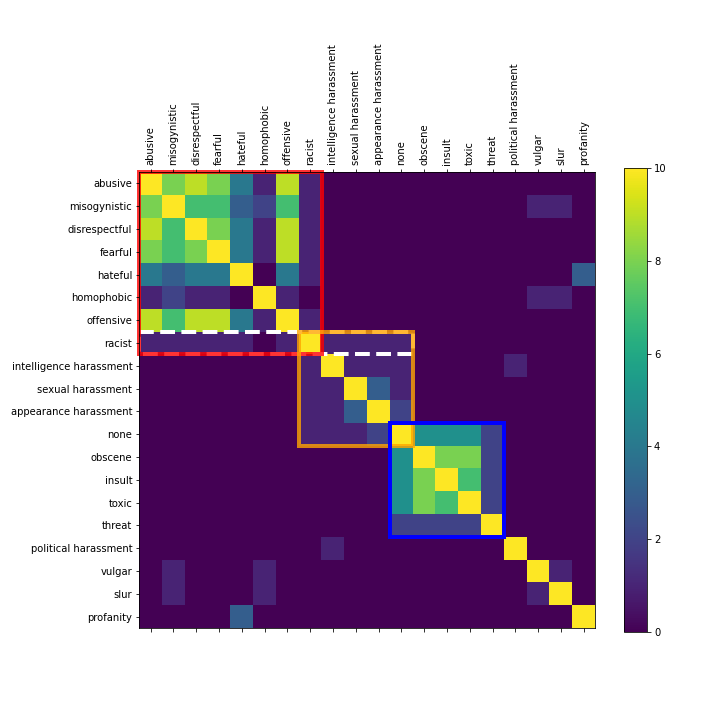
\includegraphics[width=\columnwidth]{NLP_LaTeX_Template/fig/heatmap_of_common_words.png}
    \caption{Number of common words extracted with TF-IDF.}
    \label{fig:common_tfidf}
\end{figure}
We come to the same conclusion if we use hierarchical clustering. The dendrogram can be seen in figure \ref{fig:hierarchical_tfidf}.
\begin{figure}
    \centering
    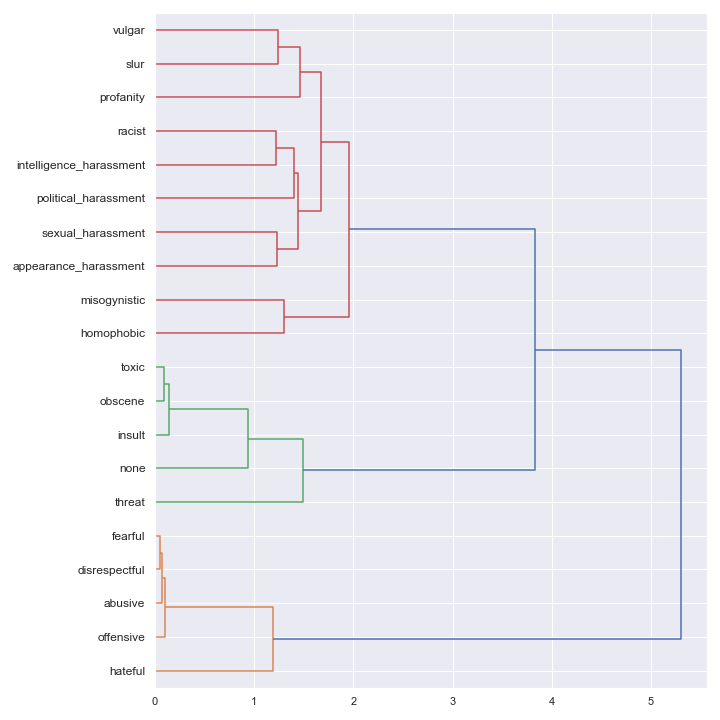
\includegraphics[width=\columnwidth]{NLP_LaTeX_Template/fig/tf-idf_cluster.png}
    \caption{30 important words extracted for each label with TF-IDF. Labels cluster using TF-IDF coefficients.}
    \label{fig:hierarchical_tfidf}
\end{figure}

We used word embeddings from TF-IDF coefficients for the most important words for each label according to TF-IDF. 2D projection can be seen in figure \ref{fig:tfidf_embedding}.
\begin{figure}
    \centering
    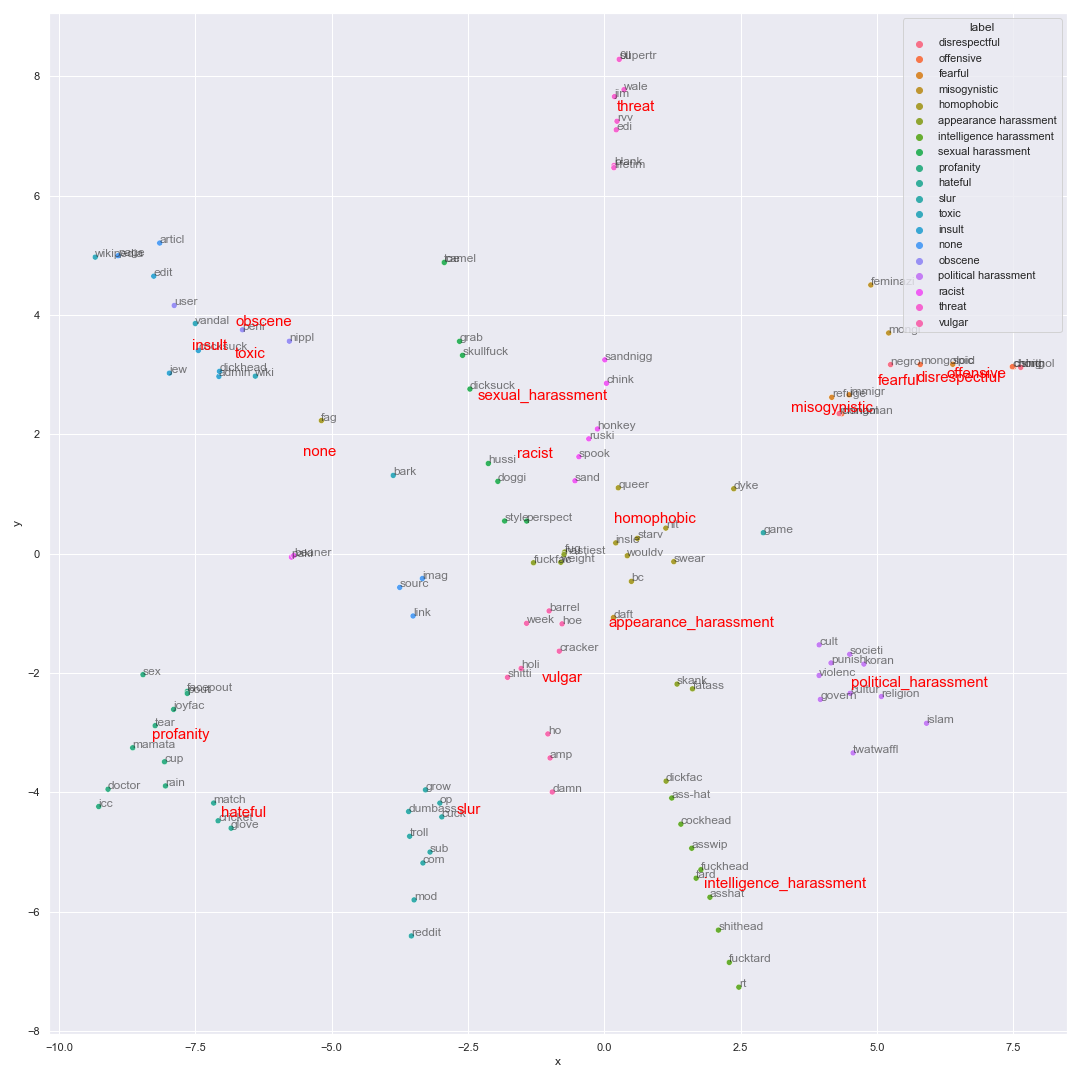
\includegraphics[width=\columnwidth]{NLP_LaTeX_Template/fig/TSNE-tfidf.png}%[width=\columnwidth]
    \caption{Important words embedded with t-SNE using TF-IDF coefficients.}
    \label{fig:tfidf_embedding}
\end{figure}
We can observe that appearance and intellectual harassment are in the same cluster. The same is with obscene and insult. But there are also clusters that stands for it own such as slur, threat, profanity and threat.

To project data to 2D we also used LDA (Linear Discriminant Analysis), which does not only use embeddings but also the words label. We used only the words with one label out of the most important ones. The projection can be seen in figure \ref{fig:fasttext_LDA}.
\begin{figure}
    \centering
    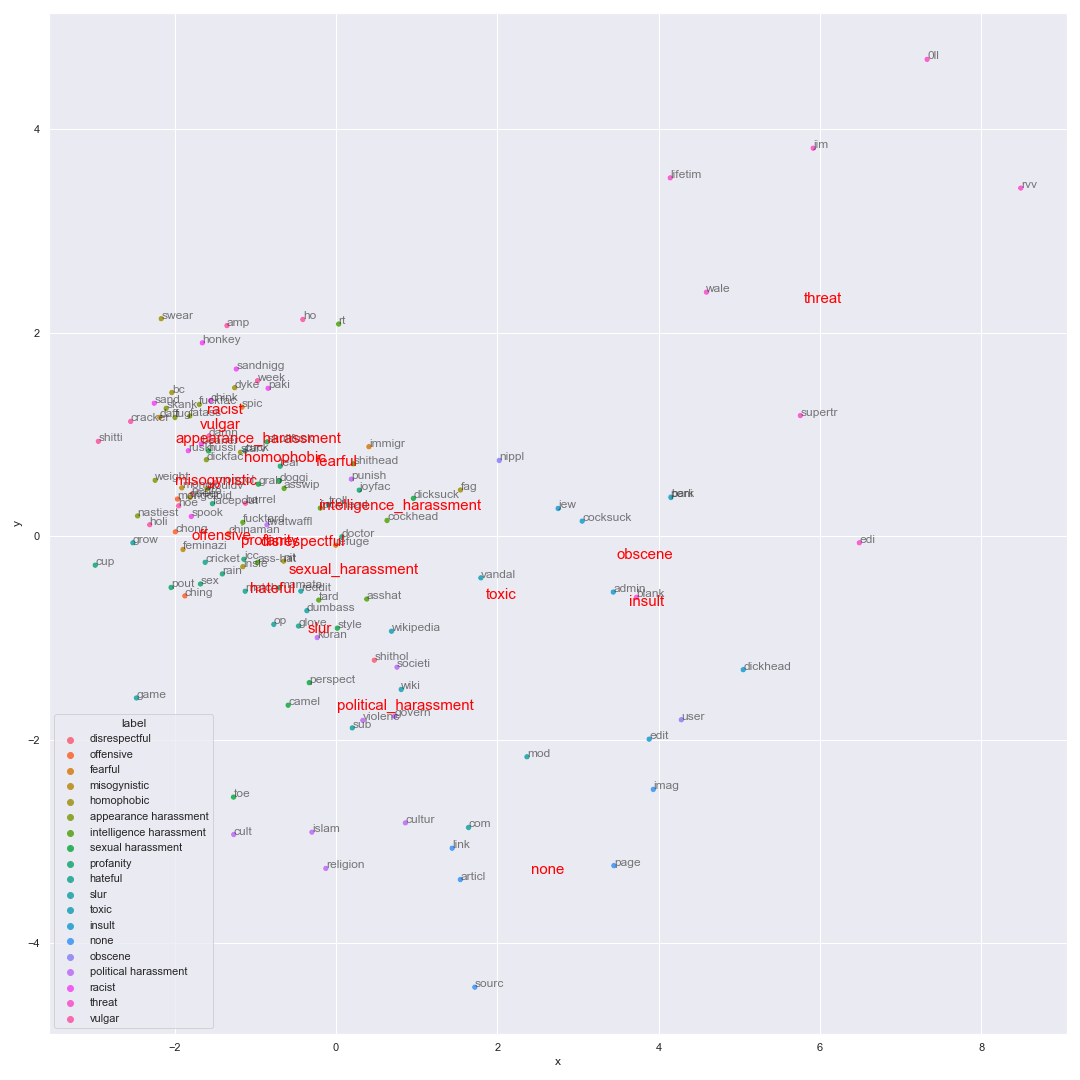
\includegraphics[width=\columnwidth]{NLP_LaTeX_Template/fig/LDA-fasttext.png}%[width=\columnwidth]
    \caption{Important words embedded with FastText and projected using LDA.}
    \label{fig:fasttext_LDA}
\end{figure}
Most important observation we can make is that the label none is separable from all of the other labels, which is to be expected. Political harassment seems differs from other labels, as it is a bit further away from the central cluster. We would probably tend to say the same if we had to judge it subjectively. Racist, vulgar and appearance harassment are very similar to each other with similar words such as "dickface".

% Word2Vec
We trained our own Word2Vec model and also use some pretrained(such as word2vec-google-news-300) ones, but the embeddings were not informative. We were not able to recognize any clusters or structure in the data. The reason is probably the fact that our corpus is not large enough, to make good estimate of the weights. Another problem is that most of data are tweets and sentences are semantically poor. 

%FastText
When we used the FastText model we trained it on the whole corpus but took only the labels embeddings, and reduced its dimensionality with PCA and plotted it on a 2D plane. The results are shown on Figure~\ref{fig:fasttextpca}. From the figure a few clusters can be seen. As we can see we have a cluster with vulgarity, profanity, slur and fearful, which mostly makes sense as the labels tend to have a similar meaning. Another cluster is none and abusive, which does not make sense. We could explain this only by assuming that this embedding shows us some of the underlying bias of our corpus (at least for this two labels), In the centre of the coordinate system we have a slightly bigger cluster, with different types of harassment, offensive, disrespectful, hateful and misogynistic. The common line with this labels is that they tend to focus on the "outside" or the "inside" properties of the victim. Homophobic, racist, insult and threat are laying outside of these clusters.
\begin{figure}
    \centering
    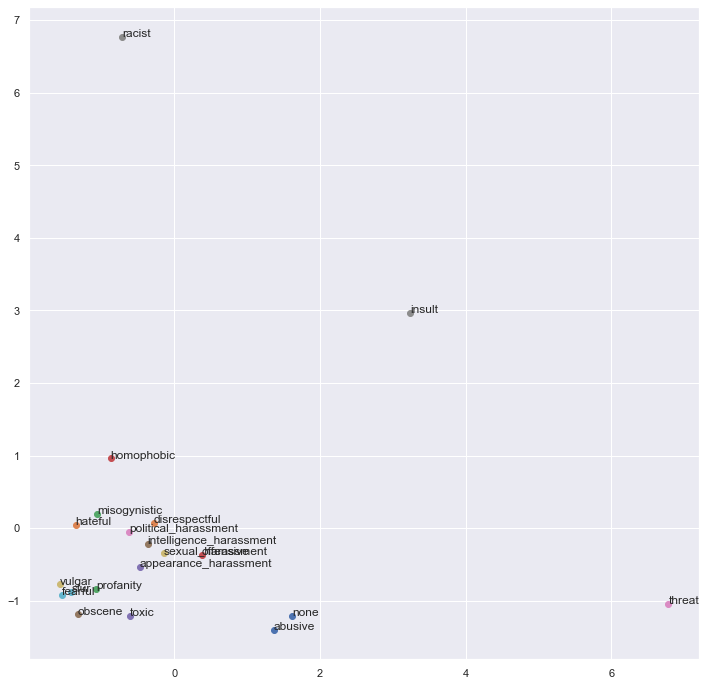
\includegraphics[width=0.7\columnwidth]{NLP_LaTeX_Template/fig/fastText_PCA.png}
    \caption{PCA decomposition of FastText embeddings for each label. FastText was trained on the merged dataset.}
    \label{fig:fasttextpca}
\end{figure}

%------------------------------------------------
FastText was also used to find most similar words to labels. Embedding can be seen in figure \ref{fig:fasttext_embedding}.
\begin{figure*}
    \centering
    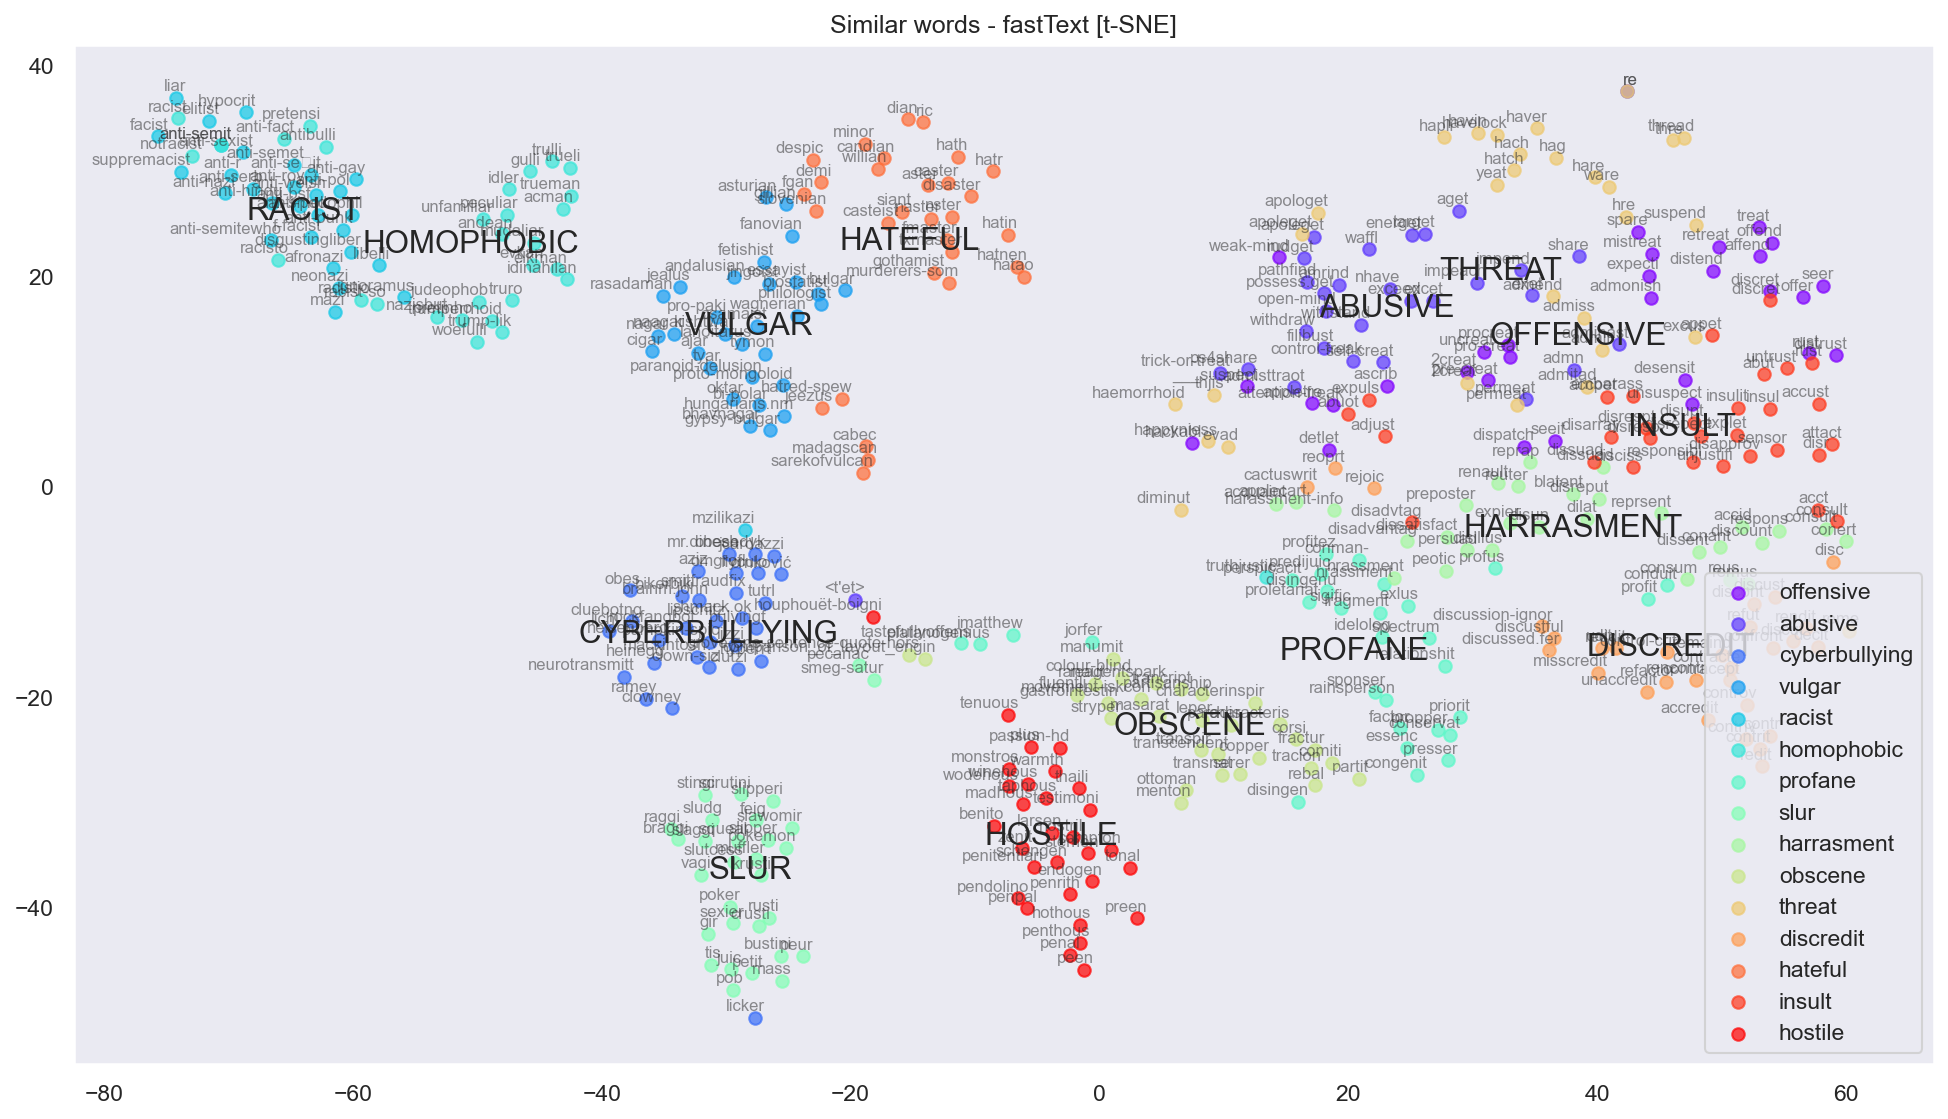
\includegraphics[width=\textwidth]{NLP_LaTeX_Template/fig/SimilarWords - fastText - t-SNE.png}
    \caption{Most similar words retrieved by fastText.}
    \label{fig:fasttext_embedding}
\end{figure*}
For some labels we get exquisite results. For instance, with the label racist we get that some of the most similar words are "neonazi","anti-semit", "facist" etc. But for many other labels most similar words do not make a lot of sense. Most of the labels are separable from the others and forms compact clusters such as slur, cyberbullying, vulgar, hateful, obscene etc. But there are labels which are very similar. For instance threat, abusive, offensive. For the compact ones we are able to say that most probably these labels cover their own area of swear words.

\section*{Future work}
In the future we will use embeddings of the most important words for each labels, returned to us by the last layer of different pretrained BERT\cite{bert-toxccin, hasoc2020} and ELMO\cite{ElmoSemEval}. With these embeddings we will try different methods of clustering and from all of the information we gathered through all of our experiments and tried to make a schema of the labels \cite{latentDirichtlet, lda2} we have in our corpus and the schema for all of the prescribed labels using similar approaches such as.

%----------------------------------------------------------------------------------------
%	REFERENCE LIST
%----------------------------------------------------------------------------------------
\bibliographystyle{unsrt}
\bibliography{report}


% \section*{Appendix}

\begin{table*}[ht]
\centering
\begin{tabular}{l|rrrrrrr|r}
Sentiment & 16 fcbk & 20 twtr & 25 twtr & 32 twtr & wikipedia & vulgar twtr & reddit & total \\
\midrule
  %\hline
  abusive &   0 & 671 &   0 &   0 &   0 &   0 &   0                   & 671   \\ 
  appearance\_harassment &   0 &   0 &   0 & 677 &   0 &   0 &   0    & 677   \\ 
  disrespectful &   0 & 782 &   0 &   0 &   0 &   0 &   0             & 782   \\ 
  fearful &   0 & 562 &   0 &   0 &   0 &   0 &   0                   & 562   \\ 
  hateful &   0 & 1278 & 1267 &   0 &   0 &   0 &   0                 & 2545  \\ 
  homophobic &   0 & 845 &   0 &   0 &   0 &   0 &   0                & 845   \\ 
  insult &   0 &   0 &   0 &   0 & 7877 &   0 &   0                   & 7877  \\ 
  intelligence\_harassment &   0 &   0 &   0 & 810 &   0 &   0 &   0  & 1360  \\ 
  misogynistic &   0 & 1360 &   0 &   0 &   0 &   0 &   0             & 33157 \\ 
  none &   0 &   0 & 4456 & 21059 & 7642 &   0 &   0                  & 810   \\ 
  obscene &   0 &   0 &   0 &   0 & 8449 &   0 &   0                  & 8449  \\ 
  offensive &   0 & 4020 & 522 &   0 &   0 &   0 &   0                & 4542  \\ 
  political\_harassment & 3864 &   0 &   0 & 698 &   0 &   0 &   0    & 4562  \\ 
  profanity &   0 &   0 & 760 &   0 &   0 &   0 &   0                 & 760   \\ 
  racist &   0 &   0 &   0 & 702 &   0 &   0 &   0                    & 702   \\ 
  sexual\_harassment &   0 &   0 &   0 & 229 &   0 &   0 &   0        & 229   \\ 
  slur &   0 &   0 &   0 &   0 &   0 &   0 & 5059                     & 5059  \\ 
  threat &   0 &   0 &   0 &   0 & 478 &   0 &   0                    & 478   \\ 
  toxic &   0 &   0 &   0 &   0 & 16889 &   0 &   0                   & 16889 \\ 
  vulgar &   0 &   0 &   0 &   0 &   0 & 6718 &   0                   & 6718  \\ 
   %\hline
  \bottomrule
  total & 3864 & 9518 & 7005 & 24175 & 41335 & 6718 & 5059            & 97674 \\
\end{tabular}
\caption{Number of documents for different sentiments and sources. Prefix numbers of sources are indexes from \url{https://hatespeechdata.com/}}
\label{tab:sentiment-source}
\end{table*}



\end{document}